% !TEX TS-program = PDFlatex
% !TEX encoding = UTF-8 Unicode

% Example of the Memoir class, an alternative to the default LaTeX classes such as article and book, with many added features built into the class itself.

%\documentclass[12pt,a4paper]{memoir} % for a long document
%\documentclass[french,12pt,a4paper,article]{memoir} % for a short document
\documentclass[english,12pt,article]{article} % for a short document
%\documentclass[french,12pt,a4paper]{article} % for a short document

\usepackage{babel}
\usepackage[utf8]{inputenc} % set input encoding to utf8
\usepackage{amsmath, amsthm, amssymb}

\input{amssym.def}
\input{amssym.tex}

% Don't forget to read the Memoir manual: memman.PDF
\usepackage{enumitem}
\usepackage{alltt}
\usepackage{color}
\usepackage{pgfplotstable}
\usepackage{pgfplots}
\usetikzlibrary{plotmarks}
\usepackage[colorlinks=true,linkcolor=blue]{hyperref} 
\usepackage{graphicx}
\usepackage{listings}
\usepackage[T1]{fontenc}   % so _, <, and > print correctly in text.
\usepackage[strings]{underscore}    % to use "_" in text
%\frenchspacing
\usepackage{pdfpages}

%%% Examples of Memoir customization
%%% enable, disable or adjust these as desired

%%% PAGE DIMENSIONS
% Set up the paper to be as close as possible to both A4 & letter:
%\settrimmedsize{11in}{210mm}{*} % letter = 11in tall; a4 = 210mm wide
%\setlength{\trimtop}{0pt}
%\setlength{\trimedge}{\stockwidth}
%\addtolength{\trimedge}{-\paperwidth}
%\settypeblocksize{*}{\lxvchars}{1.618} % we want to the text block to have golden proportionals
%\setulmargins{50pt}{*}{*} % 50pt upper margins
%\setlrmargins{*}{*}{1.618} % golden ratio again for left/right margins
%\setheaderspaces{*}{*}{1.618}
%\checkandfixthelayout 
% This is from memman.PDF

\newcommand{\latex}{\LaTeX\xspace}
\newcommand{\tex}{\TeX\xspace}
 
\def\th#1{theorem~\ref{#1}}
\def\Th#1{Theorem~\ref{#1}}
\def\eq#1{\rm Eq.~(\ref{#1})}
\def\Eq#1{\rm Eq.~(\ref{#1})}
\def\eqs#1{\rm Eqs.~(\ref{#1})}
\def\eqe#1{(\ref{#1})}
\def\sec#1{\rm Sec.~(\ref{#1})}
\def\secs#1{\rm Secs.~(\ref{#1})}
\def\sece#1{(\ref{#1})}
\def\Fig#1{\rm Figure {\rm \ref{#1}}}
\def\fig#1{\rm Figure {\rm \ref{#1}}}
\def\fige#1{ {\rm \ref{#1}}}
\def\figs#1{\rm Figures {\rm \ref{#1}}}

\definecolor{darkgreen}{rgb}{0,0.8,0.2}
\definecolor{mauve}{rgb}{0.88,0.69,1.0}
\definecolor{morve}{rgb}{0.58,0.7,0.39}
\definecolor{darkred}{rgb}{0.58,0.0,0.0}
%\definecolor{ered}{rgb}{1.0,0.0,0.0}
\definecolor{ered}{rgb}{0.0,0.0,0.0}   % ered devient noir
\definecolor{pion}{rgb}{0.01.0,1.0}

\newcommand\dottcmd[1]{\texttt{#1}\endgroup}
\newcommand{\vn}{\begingroup\catcode`\_=11 \catcode`\%=11 \dottcmd}

\newenvironment{example}
  {\vspace{-2.5ex}\small \begin{alltt}}
  {\end{alltt} \vspace{-2.0ex}}

\newenvironment{example1}
  {\vspace{-2.0ex}\footnotesize \begin{alltt}}
  {\end{alltt} \vspace{-1.5ex}}

\newenvironment{example2}
  {\vspace{-2.0ex}\scriptsize \begin{alltt}}
  {\end{alltt} \vspace{-1.5ex}}

\definecolor{light-gray}{gray}{0.95}
\lstset{backgroundcolor=\color{light-gray}}
\lstset{xleftmargin=0cm}
\lstset{framexleftmargin=0.3em}
\lstset{basicstyle=\scriptsize}
\lstnewenvironment{code}{}{}

\newlength{\dPar}
\setlength{\dPar}{1.5ex}
\setlength{\parskip}{\dPar}
\setlength{\parindent}{0ex}

%-----------------------------------------------------------------

\title{ \protect \large Manual for FPP:   The Fully Polymorphic Package}    
\newcommand{\subtitle}{Using examples from  PTC and BMAD }
\author{Étienne Forest \\ Tsukuba, Japon }
%\date{12 avril 2018} 
%\date{21 juillet 2018} % Delete this line to display the current date

\bibliographystyle{prsty}
  
\begin{document}
 
\maketitle

\newpage 
{\footnotesize
\tableofcontents % the asterisk means that the contents itself isn't put into the ToC
}
\newpage 

%--------------------------------------------------------------
\section{Introduction to FPP/PTC}
\label{sec:fppptc}

\begin{figure}[tb]
  \centering
  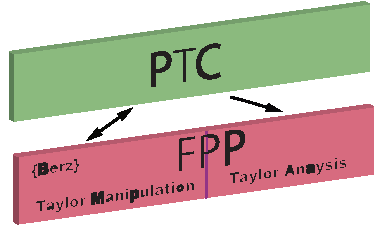
\includegraphics{FPP-PTC.pdf}
  \caption{The Fully Polymorphic Package (FPP) part of the FPP/PTC library provides manipulation and analysis of Taylor series and maps and the Polymorphic Tracking Code (PTC) part provides the physics from which accelerators can be analyzed.}
  \label{f:fpp-ptc}
\end{figure}

%--------------------------------------------------------------
\subsection{FPP and PTC}

FPP/PTC is an object oriented, open source, subroutine library for
\begin{enumerate}[itemsep=-0.5ex, topsep=-0.4ex]
\item The manipulation and analysis of Taylor series and Taylor maps.
\item Modeling of charged particle beams in accelerators using Taylor maps.
\end{enumerate}

FPP/PTC has two parts. The Fully Polymorphic Package (FPP) is the part that deals with Taylor series and maps. FPP is pure math independent\footnote{It does not contain any physical description of what an accelerator is. } of any "physics". The Polymorphic Tracking Code (PTC) part of the library deals with the modeling of particle beams and accelerators. PTC contains the "physics" and relies on FPP for producing and manipulating Taylor maps. This is illustrated in \Fig{f:fpp-ptc}. Roughly, FPP can be subdivided into two parts(see \sec{sec:subp}), a Taylor manipulation part for basic manipulations of Taylor series and an analysis part to do things like normal form analysis. PTC uses the Taylor manipulation part of FPP for things like the construction of Taylor maps. Additionally, PTC uses the analysis tools of FPP. A closer look at FPP shows the existence of a Differential Algebra (DA) package within FPP. This package was originally coded by Martin Berz.

%--------------------------------------------------------------
\subsection{Where to Obtain FPP/PTC}

%--------------------------------------------------------------
\subsection{Concepts}

FPP/PTC is written in object oriented Fortran2008. 

FPP/PTC uses double precision real numbers defined using the type "real(dp)" "dp" is defined in FPP/PTC to correspond to double precision. For example, to define in a program a real number named "time" one would write:
\begin{example}
  real(dp) time
\end{example}

In Fortran, a "structure" (also called a "derived type") is like a struct in C or a class in C++. A structure holds a set of components as defined by the programmer. With FPP, the "taylor" structure is used to hold a taylor series. For practical calculations it is often not convenient to deal directly with the taylor structure. For reasons that will be discussed later, the preferred structure to use is a polymorphic structure called "\vn{real_8}". In general, a "polymorphic" variable is a variable that can act in different ways depending on the context of the program. Here, a real_8 variable can act as if it were a real number or it can act as if it were a Taylor series depending upon how it is initialized.
An example program will make this clear.
\begin{code}
  program real_8_example
  use pointer_lattice   ! Read in structure definitions, etc.
  implicit none

  type (real_8) r8      ! Define a real_8 variable named r8
  real(dp) x            ! Define a double precision number

  !

  longprint = .false.         ! Shorten "call print" output
  call init (only_2d0, 3, 0)  ! Initialize: #Vars = 2, Order = 3

  x = 0.1d0
  call alloc(r8)          ! Initialize memory for r8
  r8 = x                  ! This will make r8 act as a real

  print *, 'r8 is now acting as a real:'
  call print (r8)

  r8 = 0.7d0 + dz_8(1) + 2*dz_8(2)**3 ! Init r8 as a Taylor series
  print *, 'r8 is now acting as a Taylor series:'
  call print(r8)

  r8 = r8**4  ! Raise the Taylor series to the 4th power
  print *, 'This is r8^4:'
  call print (r8)

  call kill(r8)
  end program
\end{code}

The variable \vn{x} is defined as a double precision real number. The line
\begin{example}
  type (real_8) r8
\end{example}
defines \vn{r8} as an instance of a \vn{real_8} variable and the line
\begin{example}
  call alloc(r8)
\end{example}
initializes \vn{r8}. This initialization must be done before \vn{r8} is used. After \vn{r8} is used, any memory that has been allocated for use with \vn{r8} is reclaimed by calling the \vn{kill} routine
\begin{example}
  call kill(r8)
\end{example}
Strictly speaking, the \vn{kill} is not necessary here since \vn{kill} is called at end of the program. However, in a subroutine or function, all local instances of \vn{real_8} variables must be killed otherwise there will be a memory leak.

When \vn{r8} is set to the real number \vn{x} in the line
\begin{example}
    r8 = x
\end{example}
this will cause \vn{r8} to act as a real number. This is verified by printing the value of \vn{r8} in the lines
\begin{example}
  print *, 'r8 is now acting as a real:'
  call print (r8)
\end{example}
The output is just a single real number indicating that \vn{r8} is acting as a real:
\begin{example}
  r8 is now acting as a real:'
  0.100000000000000
\end{example}
Notice that the \vn{print} statement uses the Fortran intrinsic print function while the \vn{call print} statement uses the overloaded print subroutine defined by \vn{FPP}.

When \vn{r8} is set to a Taylor series in the line
\begin{example}
  r8 = 0.7d0 + dz_8(1) + 2*dz_8(2)**3 ! Init r8 as a Taylor series
\end{example}
this will cause \vn{r8} to act as a Taylor series. To understand how this initialization works, first consider the initialization of FPP/PTC which was done by the line
\begin{example1}
  call init (only_2d0, 3, 0)  ! Initialize FPP/PTC. #Vars = 2, Order = 3
\end{example1}
The first argument, \vn{only_2d0},  configured FPP/PTC to construct any Taylor series as a function of two variables. These two variables will be called $z_1$ and $z_2$ here. The second argument, \vn{3}, gives the order at which the Taylor series is truncated to. That is, after this initialization, all Taylor series $t$ will be of the form
\begin{equation}
    t = \sum_{i,j}^{0 \le i+j \le 3} C_{ij} \, z_1^i \, z_2^j
\end{equation}
In the above initialization of \vn{r8}, \vn{dz_8(1)} represents the variable $z_1$ and \vn{dz_8(2)} represents the variable $z_2$. Thus \vn{r8} is initialized to the Taylor series
\begin{equation}
    t = 0.7 + z_1 + 2 \, z_2^3
\end{equation}
This is confirmed by printing \vn{r8} after it has been set via the lines
\begin{example}
  print *, 'r8 is now acting as a Taylor series:'
  call print(r8)
\end{example}
The output is:
\begin{example}
  r8 is now acting as a Taylor series:
  Properties, NO =    3, NV =    2, INA =   21
   *********************************************

     0  0.7000000000000000       0  0
     1   1.000000000000000       1  0
     3   2.000000000000000       0  3
\end{example}
Each line in the above output, after the line with the asterisks, represents one term in the Taylor series. The general form for printing a Taylor term is:
\begin{example}
  <term-order>   <term-coefficient>    <z1-exponent>  <z2-exponent>
\end{example}
The <term-order> is the order of the term. That is, the sum of the exponents. For example, the last line in the above printout is
\begin{example}
   3   2.000000000000000       0  3
\end{example}
and this line represents the term $2 \, z_1^0 \, z_2^3$. 

Once \vn{r8} has been initialized, it can be used in expressions. Thus the line
\begin{example}
  r8 = r8**4  ! Raise the Taylor series to the 4th power
\end{example}
raises \vn{r8} to the 4th power and puts the result back into \vn{r8}. This is confirmed by the final print which produces
\begin{example}
  This is r8^4:
  Properties, NO =    3, NV =    2, INA =   23
  *********************************************

    0  0.2400999999999999       0  0
    1   1.372000000000000       1  0
    2   2.940000000000000       2  0
    3   2.800000000000000       3  0
    3   2.743999999999999       0  3
\end{example}
Notice that the map has been truncated so that no term has an order higher than 3 as expected. Expressions using \vn{real_8} variables involve overloaded operators as discussed in section \sec{sec:over}.

%--------------------------------------------------------------
\subsection{Real\_8 Under the Hood}\label{sec:real8}

The particulars of how the \vn{real_8} structure is defined are generally not of interest to the general user. But it is instructive to take a quick look. In the \vn{FPP} code the \vn{real_8} structure is defined as:
\begin{example1}
  TYPE REAL_8
     TYPE (TAYLOR) T      !  USED IF TAYLOR
     REAL(DP) R           !    USED IF REAL
     INTEGER KIND  !  0,1,2,3 (1=REAL,2=TAYLOR,3=TAYLOR KNOB)
     INTEGER I   !   USED FOR KNOBS AND SPECIAL KIND=0
     REAL(DP) S   !   SCALING FOR KNOBS AND SPECIAL KIND=0
     LOGICAL(LP) :: ALLOC  1 IF TAYLOR IS ALLOCATED IN DA-PACKAGE
  END TYPE REAL_8
\end{example1}
The \vn{t} component of the structure is of type \vn{taylor} and is used if a \vn{real_8} variable is acting as a Taylor series. The \vn{r} component is used if a \vn{real_8} variable is acting as a real number. The \vn{kind} component is an integer that sets the behavior of a \vn{real_8} variable. Besides behaving as \vn{real} or a \vn{Taylor series}, a \vn{real_8} variable may behave as a "\vn{knob}" which will be explained later.

The \vn{real_8} structure contains a component of type \vn{taylor}. The definition of the taylor structure is
\begin{example1}
  TYPE TAYLOR
     INTEGER I       !  integer I is a pointer in old da-package of Berz
  END TYPE TAYLOR
\end{example1}
The component \vn{i} is a pointer to the differential algebra package of Berz that is contained in FPP. The details of how a Taylor series is stored in the structure is not important here. What is important is that this structure can be used to hold a Taylor series.

\subsection{Fundamental polymorphic types used in any code}\label{sec:funtype}

In this section we list all the simple types that exist in FPP in order of increasing complexity. They are needed if one write a simple tracking code.

\subsubsection{Type  \protect\vn{taylor}}

\begin{example}
  TYPE TAYLOR
     INTEGER I   
  END TYPE TAYLOR
\end{example}

This type overloads the Taylor series of the original real ``DA-Package'' of Berz. Its direct use is discouraged. Tracking programs should use the real polymorph.

\subsubsection{Type \protect\vn{complextaylor}}\label{sec:complextaylor}

\begin{example}
  TYPE COMPLEXTAYLOR
     type (taylor) r
     type (taylor) i
  END TYPE COMPLEXTAYLOR
\end{example}

This complex Taylor is made of two Taylor series which represent the real and imaginary parts. Its direct use is also  discouraged as was already explained in \sec{sec:real8} .  Consider this code fragment:



\begin{code}
    type(complextaylor) z1,z2
 
    call init(2,4)
    .
    .
    .
    z1=dz_t(1)+i_*dz_t(2)

    z2=z1**2
   write(6,*) " this is z1 "
   call PRINT(z1)   
   write(6,*) " this is z2 "
   call PRINT(z2)	
\end{code}

The variable \vn{z1} is, in Leibnitz  mathematical  language, $dx+i \, dy$. The variable \vn{z2} must simply be $dx^2-dy^2+i\, 2\, dx dy$.
\begin{example1}
  this is z1

 etall    1, NO =    2, NV =    4, INA =   23
 *********************************************

    I  COEFFICIENT          ORDER   EXPONENTS
      NO =     2      NV =     4
   1   1.000000000000000       1  0  0  0
    -1   0.000000000000000       0  0  0  0

 etall    1, NO =    2, NV =    4, INA =   24
 *********************************************

    I  COEFFICIENT          ORDER   EXPONENTS
      NO =     2      NV =     4
   1   1.000000000000000       0  1  0  0
    -1   0.000000000000000       0  0  0  0
  this is z2

 etall    1, NO =    2, NV =    4, INA =   25
 *********************************************

    I  COEFFICIENT          ORDER   EXPONENTS
      NO =     2      NV =     4
   2   1.000000000000000       2  0  0  0
   2  -1.000000000000000       0  2  0  0
    -2   0.000000000000000       0  0  0  0

 etall    1, NO =    2, NV =    4, INA =   26
 *********************************************

    I  COEFFICIENT          ORDER   EXPONENTS
      NO =     2      NV =     4
   2   2.000000000000000       1  1  0  0
    -1   0.000000000000000       0  0  0  0
\end{example1}

 \subsubsection{Type \protect\vn{real_8}}  \label{sec:real8code}


This type is the most important type if you write a tracking code of respectable length.  Imagine that your code tracks in one degrees of freedom (1-d-f). Then you will push two variables through your magnets, let us call them ${\bf z}=(z_1,z_2)$. These variables will denote  the position and the tangent of an angle in our little example.  If it is our  intention to always extract a Taylor series around a special orbit, then  it would suffice to declare as \vn{taylor} only the phase space variables ${\bf z}=(z_1,z_2)$ and any temporary variables the code might used during its calculations. 

But what if we want to include some parameters, such as quadrupole strengths in the calculation? Since this is a user decision, it is best if the code decides at execution time using the type  \vn{real_8}.  This was explained already  in \sec{sec:real8} but here we provide a small complete example.

\begin{code}
program my_small_code_real_8
use polymorphic_complextaylor
implicit none
type(real_8) :: z(2)  
real(dp) :: z0(2) = (/0,0/)  ! special orbit
type(reaL_8)  :: L , B, K_q , K_s 
integer :: nd = 1 , no = 2 , np = 0 ,ip

! nd = number of degrees of freedom
! no =  order of Taylor series
! Number of extra variables beyond 2*nd

call alloc(z)
call alloc( L , B, K_q , K_s )
np=0
print * , "Give  L and parameter ordinality (0 if not a parameter)"
read(5,*) L%r , ip
np=np+ip
call make_it_knob(L,ip);  np=np+ip;
print * , "Give  B  and parameter ordinality (0 if not a parameter)"
read(5,*) K_q%r , ip
print * , "Give  K_q and parameter ordinality (0 if not a parameter)"
read(5,*) K_q%r , ip
call make_it_knob(K_q,ip);  np=np+ip;
print * , "Give  K_s and parameter ordinality (0 if not a parameter)"
read(5,*) K_s%r , ip
call make_it_knob(K_s,ip); np=np+ip;
print * , "The order of the Taylor series ?"
read(5,*) no

call init(no,nd,np) ! Initializes TPSA 

z(1)=z0(1) + dz_8(1) <--- Taylor monomial z_1 added
z(2)=z0(2) + dz_8(2) <--- Taylor monomial z_2 added

call track(z)

call print(z)

contains

subroutine track(z)
implicit none
type(real_8) :: z(2) 
 z(1)=z(1)+L*z(2) 
 z(2)=z(2)-B-K_q*z(1)-K_s*z(1)**2 
end subroutine track

end program my_small_code_real_8
\end{code}

In this little code, there is one drift of length \vn{L} followed by a multipole kick that contains a dipole of strength \vn{B}, a quadrupole of strength \vn{K_q} and a sextupole of strength \vn{K_s}. We run the code ignoring the parameters:

\begin{example2}
 Give  L and parameter ordinality (0 if not a parameter)
1 0
 Give  B  and parameter ordinality (0 if not a parameter)
0 0
 Give  K_q and parameter ordinality (0 if not a parameter)
.1 0
 Give  K_s and parameter ordinality (0 if not a parameter)
0 0
 The order of the Taylor series ?
2

 etall    1, NO =    2, NV =    2, INA =   20
 *********************************************

    I  COEFFICIENT          ORDER   EXPONENTS
      NO =     2      NV =     2
   1   1.000000000000000       1  0
   1   1.000000000000000       0  1
    -2   0.000000000000000       0  0

 etall    1, NO =    2, NV =    2, INA =   21
 *********************************************

    I  COEFFICIENT          ORDER   EXPONENTS
      NO =     2      NV =     2
   1 -0.1000000000000000       1  0
   1  0.9000000000000000       0  1
    -2   0.000000000000000       0  0
\end{example2}



The situation presented here is very similar to the  matrix codes ``Transport'' or ``Marylie''.   This little program produces Taylor series to second order in the  phase space variables ${\bf z}=(z_1,z_2)$.

However, we can now require that the multipole strengths be variables of the Taylor series without recompiling the program. In this example, we make the quadrupole strength the third variable of TPSA:  $K_q=0.1 + dz_3$.

\begin{example2}
 Give  L and parameter ordinality (0 if not a parameter)
1 0
 Give  B  and parameter ordinality (0 if not a parameter)
0 0
 Give  K_q and parameter ordinality (0 if not a parameter)
.1 1
 Give  K_s and parameter ordinality (0 if not a parameter)
0 0
 The order of the Taylor series ?
2

 etall    1, NO =    2, NV =    3, INA =   22
 *********************************************

    I  COEFFICIENT          ORDER   EXPONENTS
      NO =     2      NV =     3
   1   1.000000000000000       1  0  0
   1   1.000000000000000       0  1  0
    -2   0.000000000000000       0  0  0

 etall    1, NO =    2, NV =    3, INA =   23
 *********************************************

    I  COEFFICIENT          ORDER   EXPONENTS
      NO =     2      NV =     3
   1 -0.1000000000000000       1  0  0
   1  0.9000000000000000       0  1  0
   2  -1.000000000000000       1  0  1
   2  -1.000000000000000       0  1  1
    -4   0.000000000000000       0  0  0
\end{example2}

Again, we must emphasize that while it would have been easy here to tun with  the type \vn{taylor} for all the variables, it is totally infeasible in a real tracking code to either recompile the code or allow all parameters of the systems to be Taylor series. This is why typical matrix\footnote{This is not true of Berz's COSY INFINITY which handles variable memory of TPSA within its own internal language.} codes, not using TPSA, are limited to a small set of Taylor variables, usually the six phase space variables.

So in summary a polymorph can be as mentioned in \sec{sec:real8}:

\begin{enumerate}
 \item A real number
 \item a Taylor series with real coefficients (\vn{taylor})
 \item a knob which is a simple temporary Taylor series activated only if needed
\end{enumerate}

 \subsubsection{Type \protect\vn{complex_8}}  \label{sec:complex_8}
 
 The type  \protect\vn{complex_8} is rarely used in a tracking code since all quantities we compute are ultimately real. However once in a while it is useful to go into complex coordinates temporarily. If the type \vn{complex_8} did not exist, then a code could become extremely difficult to write. This happens a lot when Maxwell's equation is written in cylindrical coordinate. In such a case, if ${\bf z}=(x,p_x,y,p_y)$, then most intermediate calculation involve a quantity $q=x+i\,y$. Therefore it is extremely useful inside one's code to declare \vn{q} as a complex polymorph. This happens in some magnets of PTC but it is generally hidden from a normal user. 
 
 \begin{example2}
TYPE COMPLEX_8
 TYPE (COMPLEXTAYLOR) T 
 COMPLEX(DP) R
 LOGICAL(LP) ALLOC
 INTEGER KIND
 INTEGER I,J 
 COMPLEX(DP) S
END TYPE COMPLEX_8
  \end{example2}
  
 As in the case of the real polymorph, the \vn{t} component contains the complex Taylor series and the \vn{r} component contains the complex number if the polymorph is not a Taylor series. 
  
  \subsection{Type   \protect\vn{probe_8}  specific to PTC}\label{sec:codetype}

The types of \sec{sec:funtype} are useful to anyone who decides to use FPP to write his own tracking code. In fact there is nothing ``tracking'' about these types. Once could write a code to solve a problem in finance or biology using  type \vn{real_8}. But since our ultimate goal is to describe the analysis part of FPP, we need to say a little bit more about the objects a real tracking code must deal with.

The code PTC tracks the following Fortran structure:
  

  \begin{example}
    type probe_8
     type(real_8) x(6)     ! Polymorphic orbital ray
     type(spinor_8) s(3)   ! Polymorphic spin s(1:3)
     type(quaternion_8) q 
     type(rf_phasor_8)  ac(nacmax)  ! Modulation of magnet
     integer:: nac=0 !  number of modulated clocks <=nacmax
     real(dp) E_ij(6,6)   !  Envelope for stochastic radiation
           .
           .
  end type probe_8
    \end{example}

As the reader can see, it is made out of other structures which are themselves made of \vn{real_8} or simple real numbers.  I will describe each component.

 
  
  

  \subsubsection{The   x(6) component of \vn{probe_8}  }\label{sec:codetype}

 This represents the orbital part of the ray. Thus we have the following associations:
 
 \begin{itemize}
\item In PTC units, when time is used: 
%
%]|Expr|[#b @`b___})+# b'4" Chicago^: ;bP8&c0!*-="!Helvetica|:! |
%|""*|:"x,H1,Z6,I,]<c!$1(1x,L<2^$^p^x_^$^p^0_},Ly,L<2^$^p^y_^$^|
%|p^0_},L<2(""#Symbol^:#&c0  D:"&c0!*E}("$^p^0_c}},LcT"$Monaco^:$ |
%|or c:#&c0  D:"&c0!*T}}:! : -;}& b!( b"0 b#8 b$@ b%H b&P!WW}]|[
\begin{align} x(1:6)=
\left({x,{{p}_{x} \over {p}_{0}},y,{{p}_{y} \over {p}_{0}},{\Delta E \over {p}_{0}c},cT~{\rm o}{\rm r}~{\rm c}\Delta T}\right) \end{align}
\item in BMAD units
%
%]|Expr|[#b @`b___})+# b'4" Chicago^: ;bP8&c0!*-="!Helvetica|:! |
%|""*|:"x,H1,Z6,I,]<c!$1(4x,L<2^$^p^x_^$^p^0_},Ly,L<2^$^p^x_^$^|
%|p^0_},L,M"#Symbol^:#&c0  b:"&c0!*cT"$Monaco^:$ or ,M:#&c0  b:$&c0!*c|
%|:#&c0  D:"&c0!*T,L<2(":#&c0  D:"&c0!*p}^$^p^0_}}}:! : -;|
%|}& b!( b"0 b#8 b$@ b%H b&P!WW}]|[
\begin{align} x(1:6)=
\left({x,{{p}_{x} \over {p}_{0}},y,{{p}_{x} \over {p}_{0}},-\beta cT~{\rm o}{\rm r}~-\beta {\rm c}\Delta T,{\Delta p \over {p}_{0}}}\right) \end{align}
\end{itemize}
where
%
%]|Expr|[#b @`b___})*# b'4" Chicago^: ;bP8&c0!*-="!Helvetica|:! |
%|""Symbol^:"&c0  D"#*|:#&c0!*T,]T,M$^T(!ref}_:! : -;|
%|}& b!( b"0 b#8 b$@ b%H b&P!WW}]|[
\begin{align} \Delta T=
T-{T}_{ref} \end{align}

It does not take too much imagination to see that 1-d-f, 2-d-f and 3-d-f Taylor maps will be created easily with the appropriate initialization of the polymorphic \vn{probe_8}. 

  \subsubsection{The   spin and quaternion components of \vn{probe_8}  }\label{sec:code spin}

PTC, as BMAD, can track spin. There are two ways to track spin: one method uses a regular spin matrix and the other uses a quaternion.
Since there are three independent direction of spin, PTC tracks three directions: this saves time if one wants to construct a spin matrix. The three directions are represented by the three \vn{spinor_8}  called \vn{s(3)}. A \vn{spinor_8} is just

  \begin{example}
  type spinor_8
     type(real_8) x(3)  ! x(3) = (s_x, s_y, s_z)   with  |s|=1
  end type spinor_8
    \end{example}

For example if one tracks on the closed orbit, the following initial conditions
%
%]|Expr|[#b @`b___})9# b'4" Chicago^: ;bP8&c0!*-="!Helvetica|:! |
%|""*|:"s,H1,I:!,F,]<c!$1(%:"1,L0,L0}}: ;bP;/":!;bP8 :"s,H2,I:!,F,]|
%|<c!$1(%:"0,L1,L0}}: ;bP;/":!;bP8 :"s,H3,I:!,F,]<c!$1(%:"0,L0,L|
%|1}}: -;}& b!( b"0 b#8 b$@ b%H b&P!WW}]|[
\begin{align} s(1)&=\left({1,0,0}\right)\nonumber \\
 s(2)&=\left({0,1,0}\right)\nonumber \\
 s(3)&=\left({0,0,1}\right)\end{align}
the end vectors will allow us to construct  the one-turn matrix around the closed orbit. Thus if the orbital polymorphs are powered to be appropriate Taylor series in n-d-f (n=1,2, or 3), we can produce a complete approximate map for the spin: this will be discussed later.


The polymorphic  quaternion \vn{quaternion_8}, not surprisingly, is given by:
 
  \begin{example}
 type  quaternion_8 
  type(real_8) x(0:3)
end type quaternion_8
  \end{example}
   
   As we will see, it is a more efficient representation for the spin and it simplifies the analysis. From the matrix, we know that there is one invariant unit direction and one angle of rotation around this axis. The unit quaternion has exactly the same freedom: four numbers whose squares add up to one. Once more we claim that if its polymorphic components are properly initialized, a generic Taylor map for the quaternions emerges.
   
  \subsubsection{The   components of type \vn{rf_phasor_8_8}  }\label{sec:codemod}
  
  These objects are a little more complex to explain but their Fortran definition is simple:
  
     \begin{example}
  type rf_phasor_8
     type(real_8)  x(2)  ! The two hands of the clock
     type(real_8) om     ! the omega of the modulation
     real(dp) t          ! the pseudo-time
  end type rf_phasor_8
    \end{example}
    
  The variables \vn{x(2)} represents a vector rotating at frequency \vn{om} based on a pseudo-time related to the reference time of the ``design'' particle.   As the the \vn{probe_8} traverses a magnet, in the integration routines, magnets use that pseudo-clock to modulate their multipole components. In the end, as we will see, the components \vn{rf_phasor_8%x(2)} is used to add two additional dimensions to a Taylor map. This will be explained later when we discuss the types germane to analysis.
    
   \subsubsection{The   real components \vn{E_i_j(6,6)}  }\label{sec:codesto}
   
    We will say little about this except that allow us to store the quantum fluctuations due to radiation. PTC, like most codes, does not attempt to go beyond linear dynamics when dealing with photon fluctuations. When radiation is present, the polymorphs \vn{x(6)} contain the finally trajectory (with classical radiation) and   \vn{E_i_j(6,6)  } measures the fluctuations $<x_i\, x_j>\,i,j=1,6$ due to photon emission. PTC does not attempt any polymorphic computations: you get the zeroth order results around the orbit computed.
    
    
      \subsubsection{Real(dp) type   \protect\vn{probe}  specific to PTC}\label{sec:codetyper}
      
      In theory it is possible to have a code which uses the polymorphs \vn{real_8} and nothing else. However this is not what PTC does. PTC has a    \vn{real(dp)} version as well as a   \vn{real_8} embedded within itself. This is an issue of speed. 
      Consider the following Fortran statement
      
      \begin{code}
       type(real_8) a,b,c
           . 
           .
           .
           c=a+b
           .
           .
      \end{code}
      
      How many internal questions does the \vn{+} operation requires?   First it must decide if \vn{a} is real, Taylor or knob?  The same thing applies to the polymorph \vn{b}. On the basis of the answer, it must branch of 9 possibilities before it can even start to compute this sum.   This overhead slows down a polymorphic calculation even if all the variables are real.  Therefore PTC has a type \vn{probe} defined as
      
      \begin{example}
  type probe
     real(dp) x(6)
     type(spinor) s(3)
     type(quaternion) q
     type(rf_phasor)  AC(nacmax)
     integer:: nac=0
       .
       .
  end type probe
      \end{example}
      
      The components of the \vn{probe} are all analogous to the components of the \vn{probe_8} with \vn{real_8} replaced by \vn{real(dp)}. This most operations are acting directly and quickly on Fortran intrinsic types.
      
 \subsection{The type {\vn{c_taylor}}  and the Taylor maps  {\vn{c_damap}}   for analysis}
 
   PTC is an integrator  just like our little example of \sec{sec:real8code}. This little code  calls the tracking subroutine 
   \begin{code}
      subroutine track(z)
      implicit none
      type(real_8) :: z(2) 
       z(1)=z(1)+L*z(2) 
       z(2)=z(2)-B-K_q*z(1)-K_s*z(1)**2 
      end subroutine track
    \end{code}

This routines seems to compute the effect of a ``drift'' followed by a multipole ``kick'' in the jargon of accelerator physicists.  And indeed, if one substitutes it with 
   \begin{code}
      subroutine track(z)
      implicit none
      real(dp) :: z(2)            <-------- instead of type(real_8) :: z(2) 
       z(1)=z(1)+L*z(2) 
       z(2)=z(2)-B-K_q*z(1)-K_s*z(1)**2 
      end subroutine track
    \end{code}
   %
   this is indeed a trivial  drift-kick routine.   
    
It so happens that PTC tracks \vn{probe} or  \vn{probe_8}.  It is very easy to modify the above routines to reflect this fact. We insert them in a module which  uses the FPP
module \vn{tree_element_module}  where  \vn{probe} or  \vn{probe_8} are defined:

   \begin{code}
      module my_code
      use tree_element_module
      implicit none
      private trackr,trackp
      type(real_8)  :: L ,B, K_q , K_s 
      real(dp) :: L0 , B0, K_q0 , K_s0 
      real(dp) par(4)
      integer ip(4)
      
      interface track
       module procedure trackr
       module procedure trackp 
      end interface
      
      contains
                        .
                        .
                        .
      subroutine trackr(p) ! for probe
      implicit none
      type(probe) :: p
       p%x(1)=p%x(1)+L0*p%x(2) 
       p%x(2)=p%x(2)-B0-K_q0*p%x(1)-K_s0*p%x(1)**2 
      end subroutine trackr
      
      subroutine trackp(p) ! for probe_8
      implicit none
      type(probe_8) :: p
       p%x(1)=p%x(1)+L*p%x(2) 
       p%x(2)=p%x(2)-B-K_q*p%x(1)-K_s*p%x(1)**2 
      end subroutine trackp
                        .
                        .
                        .
      end module my_code
   \end{code}
    
    Then a call to \vn{track(p)} will either call 
    
    \begin{itemize} 
       \item \vn{trackr(p)} if \vn{p} is a \vn{probe}
       \item or \vn{trackp(p)} if \vn{p} is a \vn{probe_8}
     \end{itemize}  
    
    If we call  \vn{track(p)}   where \vn{p} is a  \vn{probe_8}, then the resulting   \vn{p}   could be a Taylor series which approximates the true map\footnote{The true map of the code is always what you get by calling \vn{track}.} of the code.
    
    For example, in \sec{sec:real8code}, we got the following results for the final polymorphs: 
    
    
    \begin{example1}
 Give  L and parameter ordinality (0 if not a parameter)
1 0
 Give  B  and parameter ordinality (0 if not a parameter)
0 0
 Give  K_q and parameter ordinality (0 if not a parameter)
.1 0
 Give  K_s and parameter ordinality (0 if not a parameter)
0 0
 The order of the Taylor series ?
2

 etall    1, NO =    2, NV =    2, INA =   20
 *********************************************

    I  COEFFICIENT          ORDER   EXPONENTS
      NO =     2      NV =     2
   1   1.000000000000000       1  0
   1   1.000000000000000       0  1
    -2   0.000000000000000       0  0

 etall    1, NO =    2, NV =    2, INA =   21
 *********************************************

    I  COEFFICIENT          ORDER   EXPONENTS
      NO =     2      NV =     2
   1 -0.1000000000000000       1  0
   1  0.9000000000000000       0  1
    -2   0.000000000000000       0  0
\end{example1}

It is clear that one could state from the above result:
%
%]|Expr|[#b @`b___})b A# b'4" Chicago^: ;bP8&c0!*-="!Helvetica|:! |
%|-[-<bf ""*|:"z:!-],F,]<c!$1^["" ^1^1($,M0,N1}(#0,N9}}}: ,H:! |
%|$^"#Times|:#z^1_:! -<cr $^:#z^2_:! : ,I:#,K O: ,H$^:#z_^2: ,I|
%|:! : ;8/<:";bP8eq,Zlin1: ;8/=;bP8-;}& b!( b"0 b#8 b$@ b%H b&P!WW}]|[
\begin{align} {\bf z}&=\left({\begin{array}{cc}1&1\\
-0.1&0.9\end{array}}\right)\left({\begin{array}{c} {z}_{1} \cr {z}_{2} \end{array}}\right)+\ O\left({\begin{array}{c}{z}^{2}\end{array}}\right) \label{eq:lin1}\end{align}

Therefore we could say that ${\bf z}$ or equivalently a \vn{probe_8} containing the same information is a Taylor map. But this is not done in PTC for several reasons:

\begin{enumerate}
\item The variables  $(z_1,z_2)$ could   infinitesimal with respect to machine parameters, in which case any attempt to concatenate the matrix is pure nonsense 
\item\label{item:st}  One should not confuse a set with an algebraic structure which acts on the said set.
\end{enumerate}

Item \ref{item:st} requires an explanation. Take for example  a pair of real numbers from the set  $\mathbb{R} \times \mathbb{R}$.  A priori we have no idea what structures are imposed on this pair of numbers. Indeed the structure could be    a complex number field, a one-dimensional complex vector space, a two dimensional real vector space, a twice infinite dimensional  vector space on the field of rationals, etc... In a code (or in a mathematical article), we could decide to  distinguish these structures by using a different ``plus'' sign depending on the structure: $+$ if complex numbers and say a $\oplus$ if they are vectors. 

The solution in FPP is to define  a new type and  keep the $+,*,\ldots $ signs for this new type.  Therefore we do not allow the concatenation of \vn{probe_8} even when it is reasonable. Instead we construct a map, type \vn{c_damap}, only and only if this construction is meaningful.  FPP does not prevent the construction of meaningless Taylor maps. PTC on the other hand does if the rules between the \vn{probe_8} and \vn{c_damap}  types are religiously\footnote{Neither FPP, nor PTC nor  BMAD prevents  a user to do crazy things and shove a  \vn{probe_8} into a \vn{c_damap}  anyway he sees fit. But beware of the results.}  observed.  This will now be explained before we actually describe all the operators available.

  \subsubsection{The type {\vn{c_taylor}} and the complex Berz's package }
  
  The reader will notice two seemingly identical Fortran files : \vn{c_dabnew.f90} and  \vn{cc_dabnew.f90}. The first package creates and manipulates real Taylor series. In other words, the coefficients of the monomials are \vn{real(dp)}. 
  The complex objects of \secs{sec:complextaylor} and  \sece{sec:complex_8} are made of two real type \vn{taylor}  or  \vn{real_8}  respectively. The individual coefficients inside Berz' package \vn{c_dabnew.f90} are real.
  
  It turns out that this is very inconvenient in accelerator physics. when we analyze maps. Since most of our maps are stable, their diagonal form contain complex numbers. For example, the map  of \eq{eq:lin1} can be diagonalize 
  into:
%
%]|Expr|[#b @`b___})8# b'4" Chicago^: ;bP8&c0!*-="!Helvetica|:! |
%|""Symbol^:"&c0  L"#*|:#&c0!*,]<c!$1^["" (#:!-<exp<c!$1($:#,Mi|
%| :"&c0  m}}}^:#&c0!*0^0(#:!-<exp<c!$1($:# i :"&c0  m}}}}}"$Monaco^:$&c0!* |
%|where :"&c0  m:#&c0!* ,] 0,N317560429291521:! : ;8/<:#;bP8eq,Z|
%|lam: ;8/=;bP8-;}& b!( b"0 b#8 b$@ b%H b&P!WW}]|[
\begin{align} \Lambda =
\left({\begin{array}{cc}\exp\left({-i\ \mu }\right)&0\\
0&\exp\left({\ i\ \mu }\right)\end{array}}\right)~{\rm w}{\rm h}{\rm e}{\rm r}{\rm e}~\mu \ =
\ 0.317560429291521 \label{eq:lam}\end{align}

In fact, the output  from the code, a \vn{c_damap},   is made of two \vn{c_taylor}. Please notice that the coefficient have a real and imaginary part  corresponding to the cosine and sine of $\mu$ :

\begin{example}
           2  Dimensional map

          1, NO =    1, NV =    2, INA =  139
 *********************************************

    I  COEFFICIENT          ORDER   EXPONENTS
      NO =     1      NV =     2
   1  0.9499999999999998     -0.3122498999199199       1  0
    -1   0.000000000000000       0.000000000000000       0  0

          1, NO =    1, NV =    2, INA =  138
 *********************************************

    I  COEFFICIENT          ORDER   EXPONENTS
      NO =     1      NV =     2
   1  0.9499999999999998      0.3122498999199199       0  1
    -1   0.000000000000000       0.000000000000000       0  0
  No Spin Matrix
  c_quaternion is identity
 No Stochastic Radiation
\end{example}

Finally if FPP were to be used in electron microscopy, the eigenfunctions of $L_z$ representing symmetry around the axis of the microscope are very useful: $x \pm i y$. We can see how a complex TPSA package is almost unavoidable in the field of beam dynamics.
  
%\footnote{Of course, Berz's COSY INFINITY handles complex maps.}
\newpage
  \subsubsection{The type {\vn{c_damap}} }\label{sec:c_damap}
  
  The type  \vn{c_damap} is defined as
  
  \begin{example}
 type c_damap
   type (c_taylor) v(lnv)  
   integer :: n=0 
   type(c_spinmatrix) s 
   type(c_quaternion) q
   complex(dp) e_ij(6,6) 
 end type c_damap
  \end{example}

There is an obvious resemblance  with \vn{probe_8} which we recall is:
  \begin{example}
    type probe_8
     type(real_8) x(6)     ! Polymorphic orbital ray
     type(spinor_8) s(3)   ! Polymorphic spin s(1:3)
     type(quaternion_8) q 
     type(rf_phasor_8)  ac(nacmax)  ! Modulation of magnet
     integer:: nac=0 !  number of modulated clocks <=nacmax
     real(dp) E_ij(6,6)   !  Envelope for stochastic radiation
           .
           .
  end type probe_8
    \end{example}

The first thing one notices is that \vn{c_damap}  contains \vn{lnv=100} complex Taylor series. Indeed the analysis part of FPP does not put any limit on the dimensionality of phase space beyond \vn{lnv}. For example, if the user tracks six-dimensional phase space (as in BMAD) and adds two modulated clocks, then the component   \vn{v(lnv)} will use 10 Taylor series to represent the map leaving 90 unused. 


The \vn{c_spinmatrix} is a matrix of  \vn{c_taylor} for the three spin directions
  \begin{example}
  type c_spinmatrix
     type(c_taylor) s(3,3)
  end type c_spinmatrix
      \end{example}
and the \vn{c_quaternion} follows the polymorphic quaternion:

  \begin{example}
 type  c_quaternion
  type(c_taylor) x(0:3)
END TYPE c_quaternion
      \end{example}

 It is important to realize that  $\vn{c_damap}$ can be concatenated.  For example, the diagonal matrix $\Lambda$ of \eq{eq:lam} was obtained with the Fortran statement:
   \begin{example1}
 diag=c_phasor(-1)*normal%atot**(-1)*one_period_map*normal%atot*c_phasor()
   \end{example1}

The Fortran symbol \vn{*} is overloaded to represent the ``differential algebraic''  (DA) concatenation of five maps in this example. Basically, when we deal with operators around a closed orbit, the operators form a self-consistent differential algebra. This will include all the complicated operators we will later define: vector fields, etc \ldots

Most of perturbation theory deals with differential algebraic operators. On the other hand, it is possible to concatenate \vn{c_damap} using truncated power series algebra (TPSA). In the case of TPSA, the constant part of a map is taken into account. In that case, the map concatenation uses the symbol ``\vn{.o.}''.

A tracking code like PTC produces TPSA maps if we do not compute it around  the closed orbit because of feed down issues.  Thus most calculations of lattice functions must be preceded by a computation of the closed orbit for the obtention of a self-consistent DA map. If the maps were of infinite or very large order, then we could always deal with TPSA maps and the closed orbit search would be part of the map analysis. 

\newpage

  \subsubsection{Interaction between the worlds of probes and   Taylor maps  }
  
  Let us assume that we want to compute a \vn{probe_8}, called  \vn{polymorphic_probe}, and that we want to track it around some orbit \vn{z0=(z0(1),z0(2))}. For example, \vn{z0} might contain the closed orbit. Since PTC deals with \vn{probe}, we first stick this real initial trajectory into a real \vn{probe}, say \vn{probe0}. The syntax would be:
  
    \begin{code}
     real(dp) :: z0(2) = (/0,0/)  ! special orbit
     type(probe) :: probe0 
     type(probe_8) :: polymorphic_probe  
                  .
                  .
      probe0=z0
      polymorphic_probe = probe0    <----- initial value of polymorphic_probe
      call track(polymorphic_probe)
     \end{code}
  
  However the reader will notice that nothing is said about the initial Taylor value of  \vn{polymorphic_probe}: it will simply acquire the value of \vn{probe0}. The rays will start as real numbers and the final value of  \vn{polymorphic_probe}  after tracking will be two real numbers: no Taylor information. So how do we initialize the \vn{polymorphic_probe} correctly to obtain a map? Here is the code:
  
      \begin{code}
real(dp) :: z0(2) = (/0,0/)  ! special orbit
type(probe) :: probe0 
type(probe_8) :: polymorphic_probe  
type(c_damap) Identity, one_period_map
             .
             .
 probe0=z0
 Identity=1     <-----World of c_damap

 polymorphic_probe = probe0 + Identity   <-----probes and c_damap are mixing
 call track(polymorphic_probe)
 one_period_map=polymorphic_probe       <-----probes and c_damap are mixing
     \end{code}
  
\vn{Identity} is a \vn{c_damap}. The line \vn{Identity=1} turns it into an identity map with {\bf no} constant part. This is the differential algebraic world. 
Then  \vn{probe0} is ``added'' to \vn{Identity} and the appropriate  \vn{probe_8} is  created with the \vn{=} sign. 
  
  Finally, once the tracking is done, it returns the final value of \vn{polymorphic_probe}. Now, if we want to analyze the corresponding map, we perform the reverse assignment 
  \vn{ one_period_map=polymorphic_probe}.  
  
  Someone may wonder why we insist on adding an identity map rather than the Taylor monomials as we did in   \sec{sec:real8code}. Indeed 
   \begin{example}
   Identity=1
    \end{example}
    is equivalent to 
      \begin{example}
       Identity%v(1)=dz_c(1)
       Identity%v(2)=dz_c(2)
    \end{example}   
    and thus   \vn{dz_8(1)} and \vn{dz_8(1)} could have been added directly into the \vn{probe_8} as we did in   \sec{sec:real8code}.
          \begin{example}
       polymorphic_probe%x(1)=z0(1)+dz_8(1)
       polymorphic_probe%x(2)=z0(2)+dz_8(2)
    \end{example}


The answer will become  obvious when we discuss analysis. When we track lattice functions, linear, nonlinear, with or without spin, the initial value involves a canonical transformation. For example, \vn{Identity} would be replaced by 
\vn{normal%atot} in  \sec{sec:c_damap}.



This concludes our overview of the major types: the various Taylor types, the polymorphs, the probes of PTC and the maps which can be concatenated and analyzed.
\section{Operations on Taylor structures}


\subsection{Obsolete Types} 
\section{overloading}\label{sec:over}
\section{subpackage}\label{sec:subp}
\bibliography{nlinear}


\end{document}
